\documentclass[aspectratio=169]{beamer}
\usetheme{Madrid}
\usecolortheme{default}
\usepackage[utf8]{inputenc}
\usepackage{booktabs}
\usepackage{array}
\usepackage{graphicx}
\usepackage{tikz}
\usetikzlibrary{arrows.meta,positioning,shapes.geometric}

\definecolor{creditblue}{RGB}{22,74,117}
\definecolor{creditgreen}{RGB}{37,132,92}
\definecolor{creditorange}{RGB}{210,121,35}
\setbeamercolor{structure}{fg=creditblue}
\setbeamercolor{title}{fg=creditblue}
\setbeamertemplate{navigation symbols}{}
\setbeamertemplate{footline}{\hfill\insertframenumber{} / \inserttotalframenumber\hspace{0.4cm}\vspace{0.15cm}}
\graphicspath{{assets/}}

\title{Credit-risk MLOps pipeline}
\subtitle{From leakage-safe EDA to monitored production inference}
\author{CDP 2026}
\date{September 2026}

\newcommand{\placeholder}[2]{%
  \fbox{\parbox[c][#2][c]{0.88\linewidth}{\centering\color{gray}\Large #1\\[0.4cm]\normalsize Replace with GitHub PR and review screenshot}}%
}

\begin{document}

\frame{\titlepage}

\begin{frame}{Project outcome}
\begin{columns}[T]
\column{0.56\textwidth}
\textbf{Goal:} predict late/default payment while preserving chronological validation and operating a secure CPU-only service.
\vspace{0.25cm}
\begin{itemize}
  \item Leakage-safe scikit-learn preparation pipeline.
  \item Explainable heuristic baseline, then reproducible TPE model search.
  \item Config-driven model packaging: family and hyperparameters change without API code changes.
  \item PostgreSQL-backed inference logging, drift monitoring, JWT roles, CI/CD and SAST.
\end{itemize}
\column{0.4\textwidth}
\begin{block}{Decision convention}
\centering
Default class = \textbf{0}\\[0.15cm]
Probabilities = \textbf{[P(default), P(on-time)]}\\[0.15cm]
Training selection uses temporal validation only.
\end{block}
\end{columns}
\end{frame}

\begin{frame}{Git history: full branch graph (1/2)}
\begin{center}
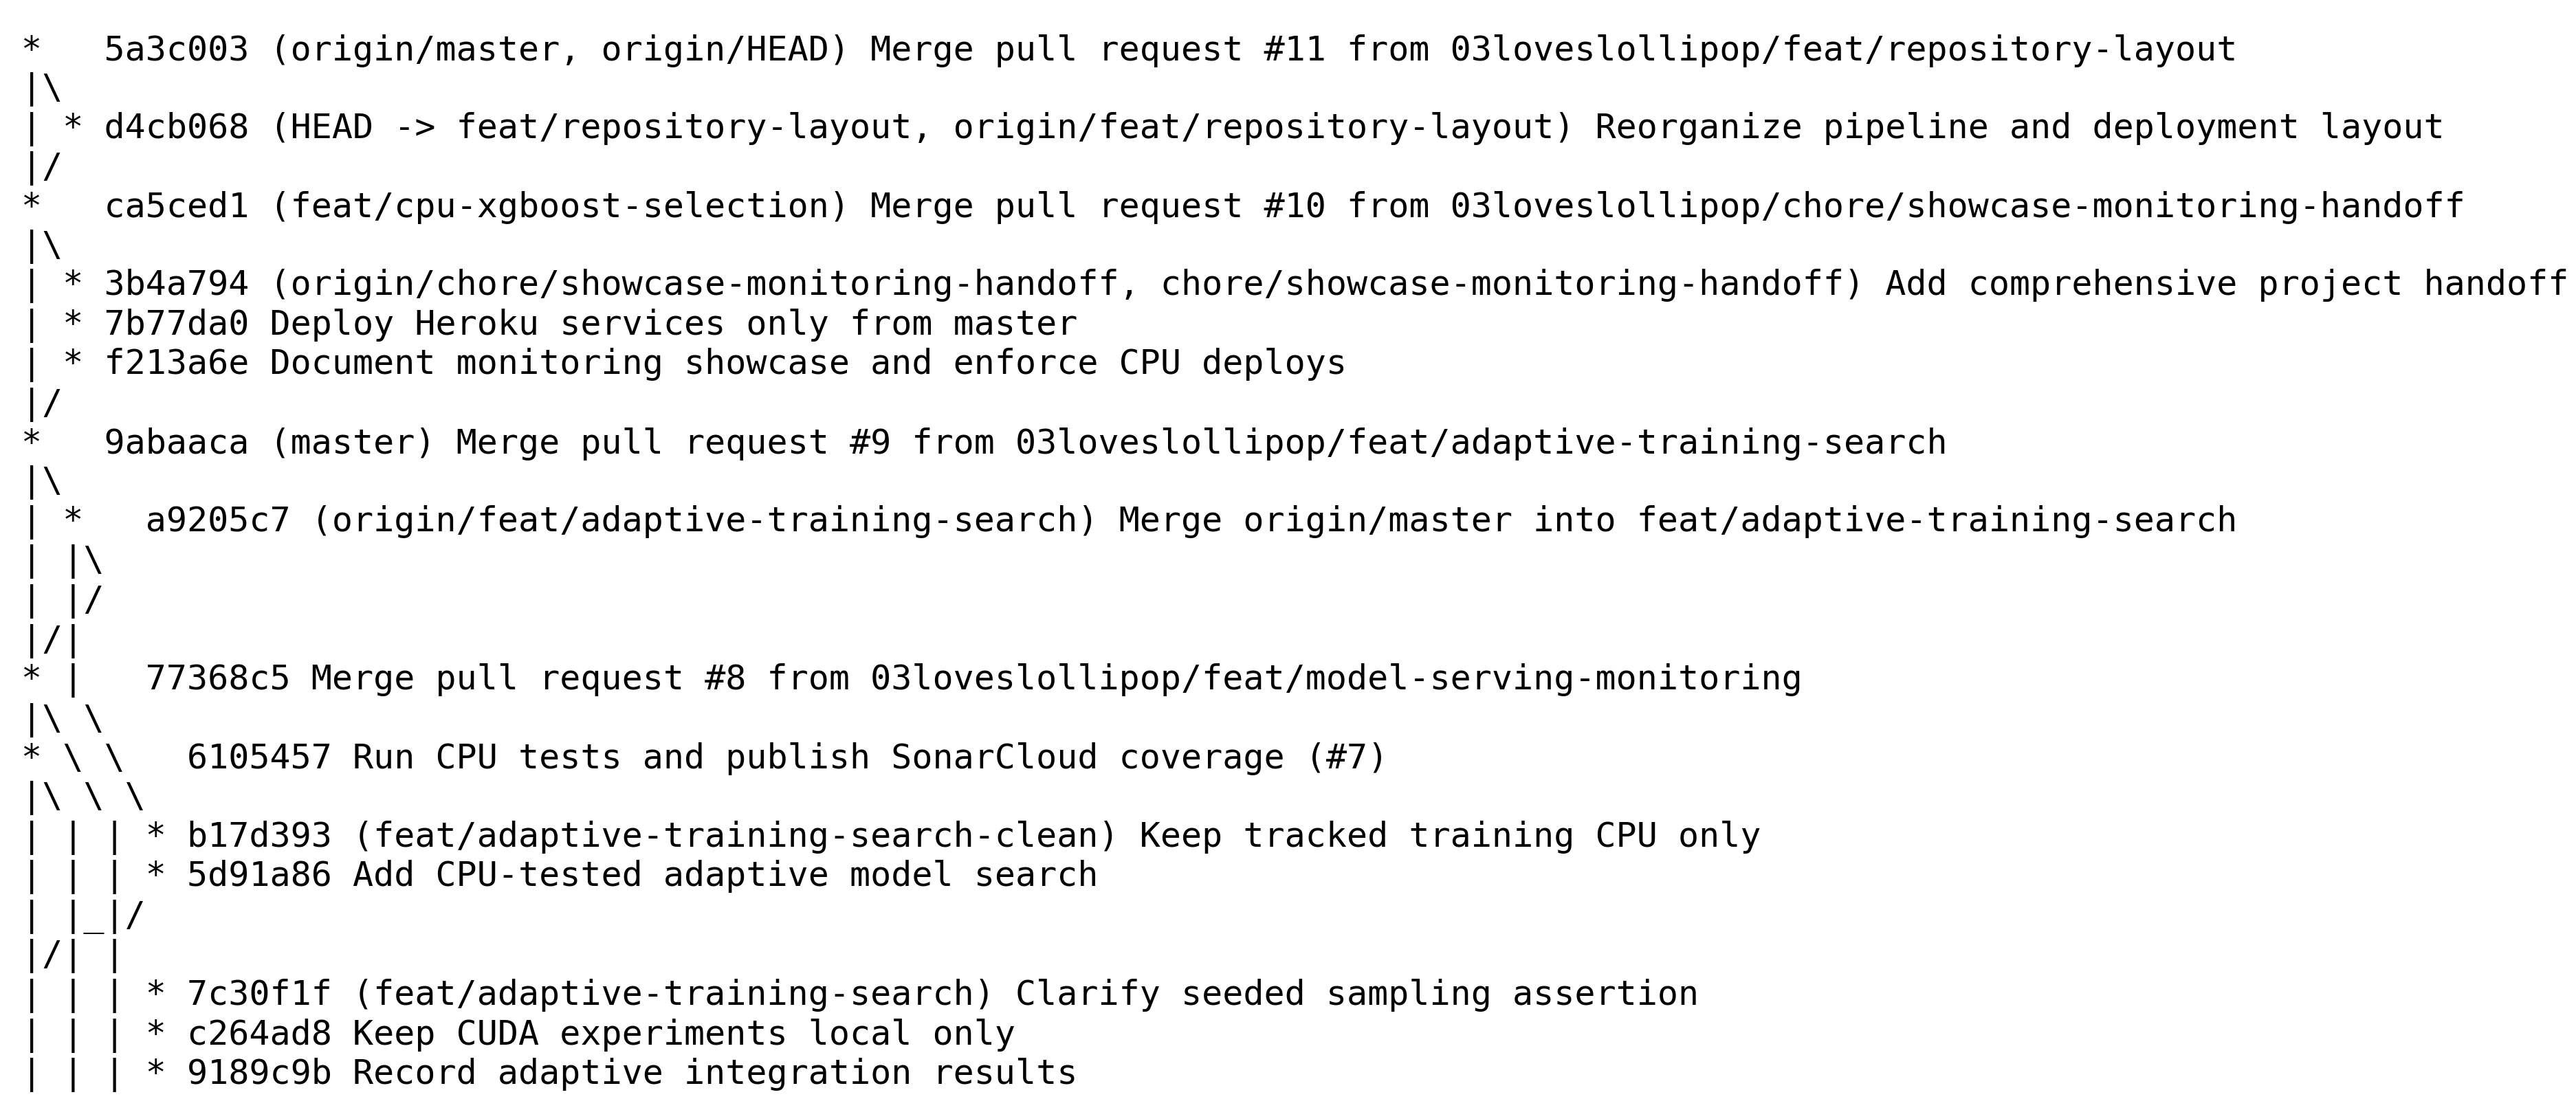
\includegraphics[width=0.98\textwidth,height=0.76\textheight,keepaspectratio]{git_graph_part_1.png}
\end{center}
\vspace{-0.2cm}
\scriptsize The graph includes all reachable branches at deck generation time. Part 2 continues on the next slide.
\end{frame}

\begin{frame}{Git history: full branch graph (2/2)}
\begin{center}
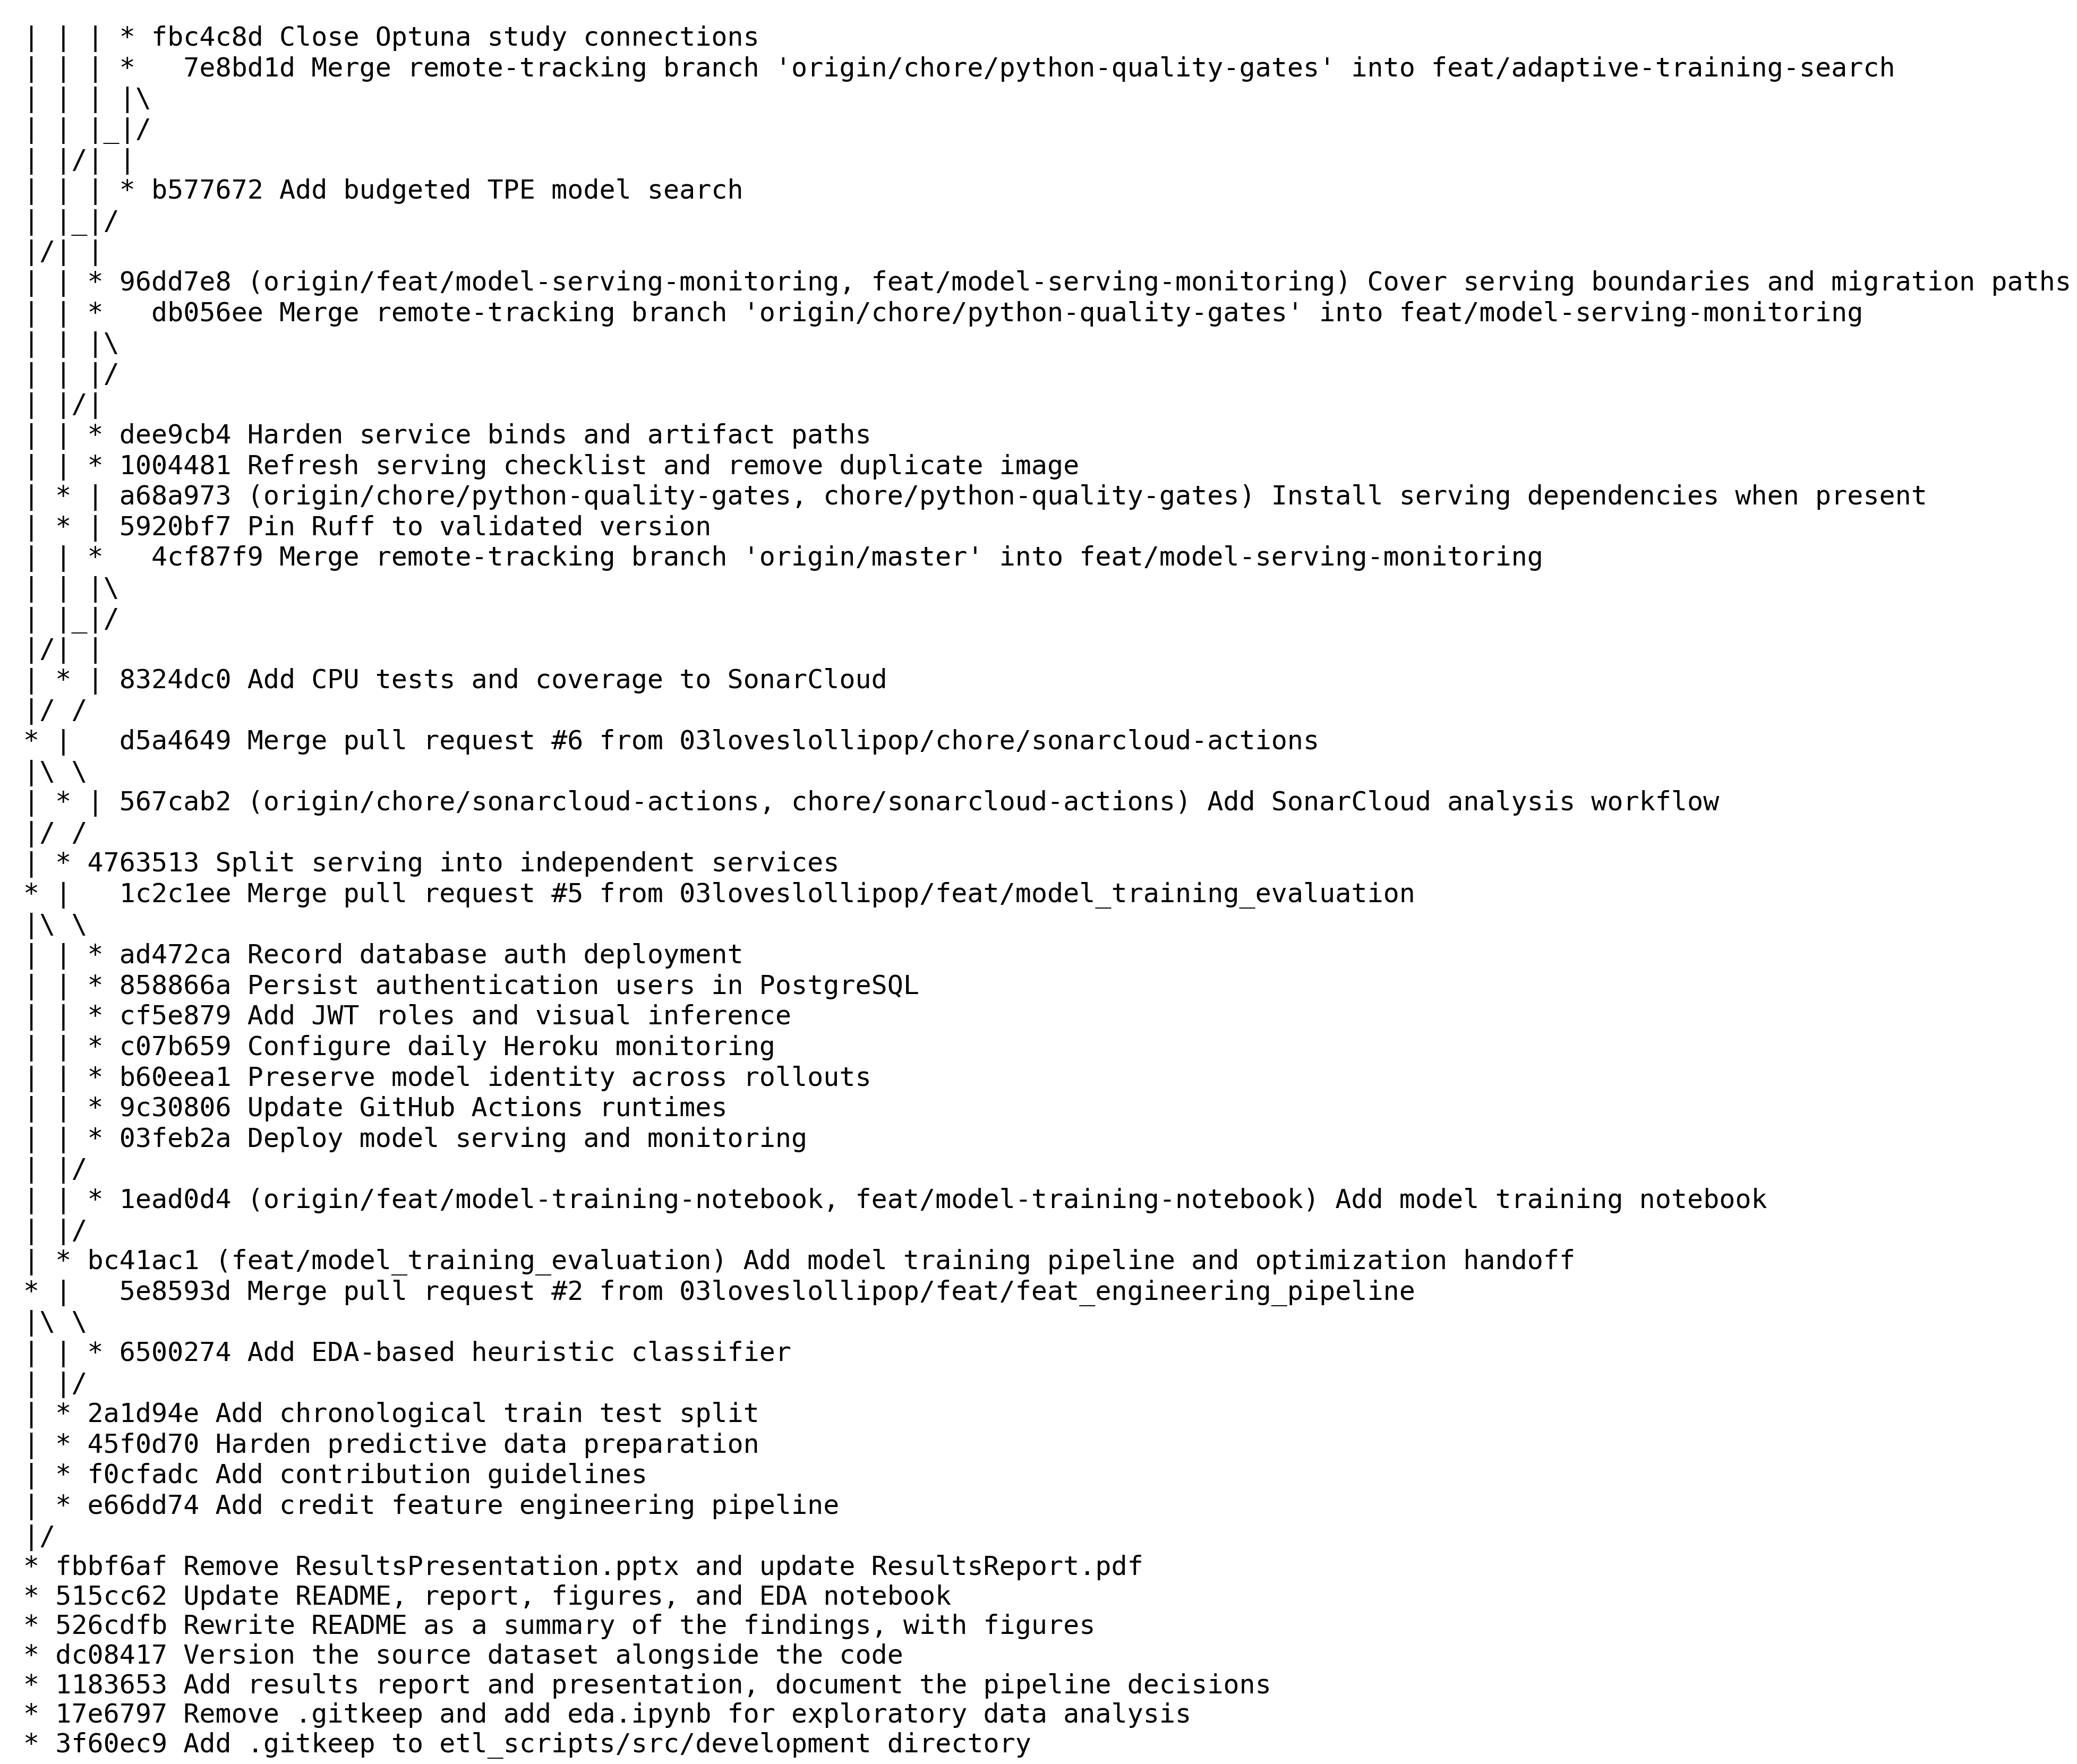
\includegraphics[width=0.98\textwidth,height=0.76\textheight,keepaspectratio]{git_graph_part_2.png}
\end{center}
\vspace{-0.2cm}
\scriptsize The highlighted review sequence and screenshot placeholders are shown next.
\end{frame}

\begin{frame}{Reviewed pull requests}
\begin{columns}[T]
\column{0.31\textwidth}
\centering\textbf{PR \#2}\\
\scriptsize Feature-engineering pipeline\\[0.15cm]
\placeholder{PR \#2 screenshot}{0.39\textheight}
\column{0.31\textwidth}
\centering\textbf{PR \#3}\\
\scriptsize Heuristic baseline into feature branch\\[0.15cm]
\placeholder{PR \#3 screenshot}{0.39\textheight}
\column{0.31\textwidth}
\centering\textbf{PR \#5}\\
\scriptsize Model training and evaluation pipeline\\[0.15cm]
\placeholder{PR \#5 screenshot}{0.39\textheight}
\end{columns}
\vspace{0.2cm}
\scriptsize PRs \#2, \#3, and \#5 are merged. Replace each panel with its GitHub PR and review screenshot before delivery.
\end{frame}

\begin{frame}{EDA and scikit-learn preparation flow}
\begin{center}
\resizebox{\textwidth}{!}{
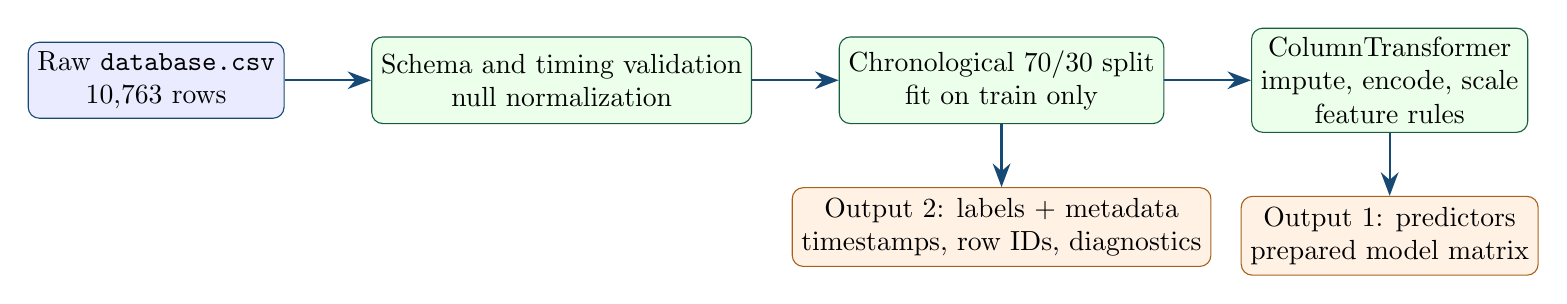
\begin{tikzpicture}[
  node distance=0.8cm and 1.1cm,
  data/.style={rectangle,rounded corners,draw=creditblue,fill=blue!8,minimum width=2.2cm,minimum height=0.9cm,align=center},
  stage/.style={rectangle,rounded corners,draw=creditgreen!70!black,fill=green!8,minimum width=2.65cm,minimum height=1.1cm,align=center},
  output/.style={rectangle,rounded corners,draw=creditorange!80!black,fill=orange!10,minimum width=2.8cm,minimum height=1cm,align=center},
  arrow/.style={-{Stealth[length=3mm]},thick,draw=creditblue}]
  \node[data] (raw) {Raw \texttt{database.csv}\\10,763 rows};
  \node[stage,right=of raw] (validate) {Schema and timing validation\\null normalization};
  \node[stage,right=of validate] (split) {Chronological 70/30 split\\fit on train only};
  \node[stage,right=of split] (prep) {ColumnTransformer\\impute, encode, scale\\feature rules};
  \node[output,below=of prep] (features) {Output 1: predictors\\prepared model matrix};
  \node[output,below=of split] (metadata) {Output 2: labels + metadata\\timestamps, row IDs, diagnostics};
  \draw[arrow] (raw) -- (validate);
  \draw[arrow] (validate) -- (split);
  \draw[arrow] (split) -- (prep);
  \draw[arrow] (prep) -- (features);
  \draw[arrow] (split) -- (metadata);
\end{tikzpicture}}
\end{center}
\vspace{0.15cm}
\small Excluded: target, bureau score leakage and metadata. Missingness indicators and validation flags are retained; no rows are silently removed.
\end{frame}

\begin{frame}{Baseline: explainable heuristic policy}
\begin{columns}[T]
\column{0.47\textwidth}
\begin{block}{What it does}
Combines EDA-derived credit signals into a transparent rule score. It is a reference policy, not a search candidate, so it anchors improvement claims.
\end{block}
\begin{tabular}{lr}
\toprule
Frozen holdout metric & Heuristic \\
\midrule
Default precision & 0.0468 \\
Default recall & 0.2685 \\
Default F1 & 0.0798 \\
Average precision & 0.0858 \\
ROC-AUC & 0.6241 \\
\bottomrule
\end{tabular}
\column{0.5\textwidth}
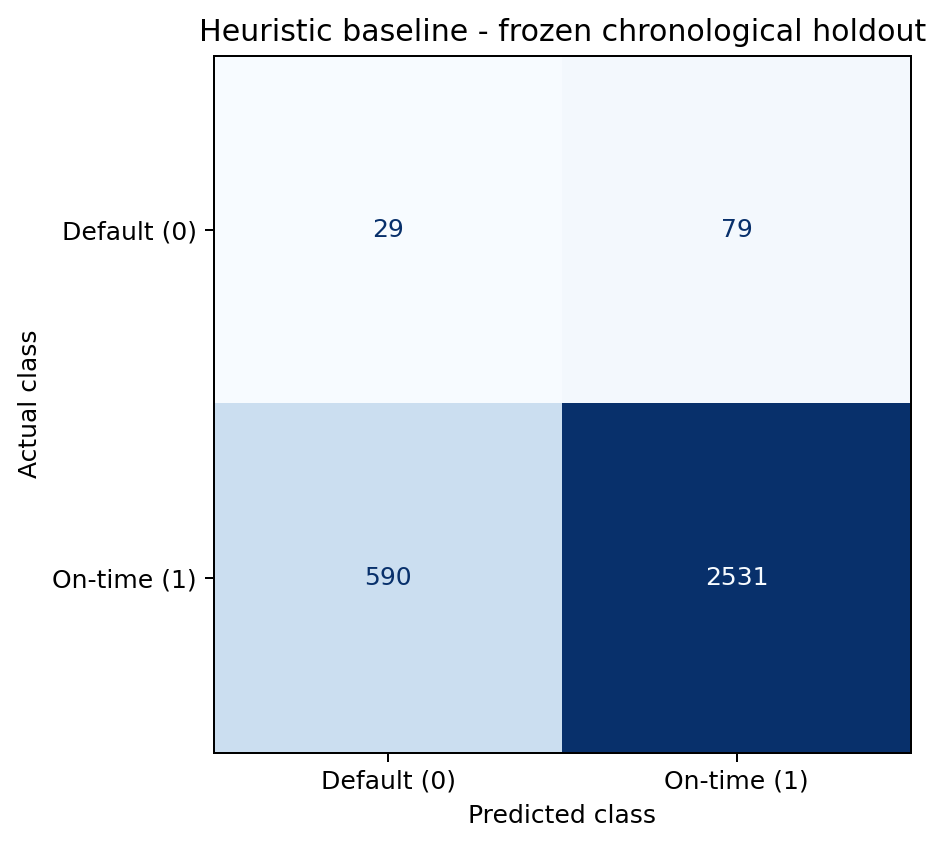
\includegraphics[width=\linewidth,keepaspectratio]{heuristic_confusion_matrix.png}
\end{columns}
\vspace{-0.22cm}
\tiny Frozen chronological holdout: 3,229 rows; default prevalence 3.34\%. Thresholds and calibration are learned from training data only.
\end{frame}

\begin{frame}{Training protocol: prevent leakage before optimizing}
\begin{center}
\resizebox{0.96\textwidth}{!}{
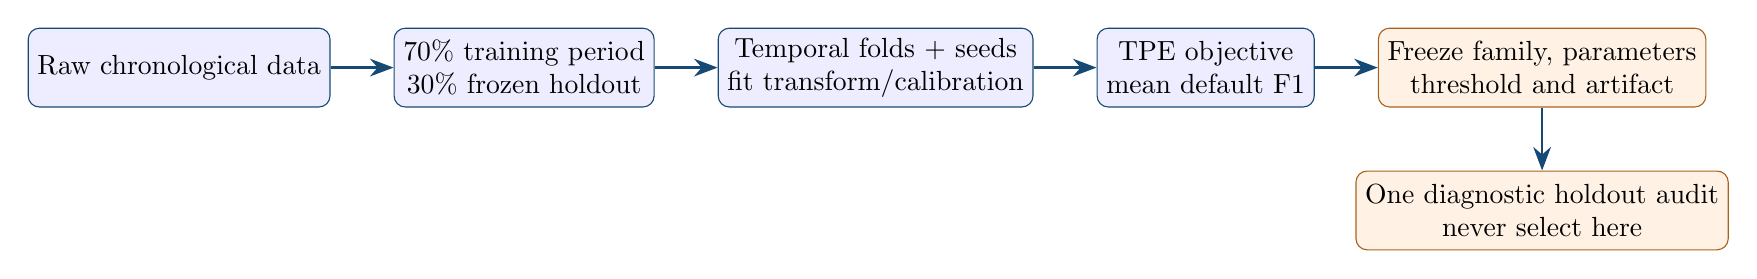
\begin{tikzpicture}[
  node distance=0.8cm and 0.8cm,
  stage/.style={rectangle,rounded corners,draw=creditblue,fill=blue!7,minimum width=2.2cm,minimum height=1.0cm,align=center},
  freeze/.style={rectangle,rounded corners,draw=creditorange!80!black,fill=orange!10,minimum width=2.3cm,minimum height=1.0cm,align=center},
  arrow/.style={-{Stealth[length=3mm]},thick,draw=creditblue}]
  \node[stage] (raw) {Raw chronological data};
  \node[stage,right=of raw] (outer) {70\% training period\\30\% frozen holdout};
  \node[stage,right=of outer] (cv) {Temporal folds + seeds\\fit transform/calibration};
  \node[stage,right=of cv] (search) {TPE objective\\mean default F1};
  \node[freeze,right=of search] (freeze) {Freeze family, parameters\\threshold and artifact};
  \node[freeze,below=of freeze] (audit) {One diagnostic holdout audit\\never select here};
  \draw[arrow] (raw)--(outer); \draw[arrow] (outer)--(cv); \draw[arrow] (cv)--(search); \draw[arrow] (search)--(freeze); \draw[arrow] (freeze)--(audit);
\end{tikzpicture}}
\end{center}
\vspace{0.2cm}
\begin{itemize}
\item Default-class F1 is primary; temporal/seed stability and CPU cost resolve close results.
\item Calibration and threshold selection use out-of-fold training scores, not holdout labels.
\end{itemize}
\end{frame}

\begin{frame}{Models tried and TPE search space}
\begin{columns}[T]
\column{0.48\textwidth}
\textbf{Learned families}
\begin{itemize}
  \item Logistic regression, decision tree, Gaussian NB, RBF SVM.
  \item Random forest and Extra Trees.
  \item XGBoost, LightGBM, PyTorch MLP.
\end{itemize}
\textbf{Reference policies}
\begin{itemize}
  \item EDA heuristic and Dummy classifier.
\end{itemize}
\column{0.48\textwidth}
\textbf{TPE controls}
\begin{itemize}
  \item 30 trials per learned family, serial/resumable SQLite study.
  \item Reproducible seed and training-only protocol fingerprint.
  \item Trees: depth/leaves, estimators, learning rate, sampling, regularization, class weights.
  \item MLP: widths, learning rate, dropout, batch size, epochs, weight decay.
\end{itemize}
\end{columns}
\end{frame}

\begin{frame}{CPU TPE rerun: strongest candidates}
\centering
\small
\begin{tabular}{lrrrrr}
\toprule
Model & F1 & temporal sd & AP & ROC-AUC & CPU batch ms \\
\midrule
Random forest & 0.2166 & 0.0333 & 0.1918 & 0.6987 & 106.0 \\
\textbf{XGBoost} & \textbf{0.2177} & 0.0238 & \textbf{0.2016} & \textbf{0.7018} & \textbf{44.6} \\
LightGBM & 0.2134 & \textbf{0.0197} & 0.1823 & 0.6897 & 52.0 \\
Heuristic & 0.1711 & 0.0223 & 0.1443 & 0.6620 & 52.4 \\
\bottomrule
\end{tabular}
\vspace{0.35cm}
\begin{block}{Interpretation}
XGBoost leads F1, AP, ROC-AUC and CPU latency. LightGBM has lower temporal variation. The deployed contract remains the validated XGBoost configuration; the latest selector's stability weighting is a documented governance decision to revisit, not a holdout-driven model swap.
\end{block}
\end{frame}

\begin{frame}{Model comparison visuals}
\begin{columns}
\column{0.5\textwidth}

\includegraphics[width=\linewidth]{temporal_f1.png}\\[0.1cm]
\centering\scriptsize Temporal-validation F1
\column{0.5\textwidth}

\includegraphics[width=\linewidth]{f1_inference_cost.png}\\[0.1cm]
\centering\scriptsize F1 versus CPU inference cost
\end{columns}
\end{frame}

\begin{frame}{Selected deployment contract: XGBoost}
\begin{columns}[T]
\column{0.5\textwidth}
\begin{block}{Config-driven release}
\texttt{deployment\_model\_config.json} contains the family, fixed hyperparameters, CPU-only runtime, class order and batch limit. The release workflow trains the configured family and packages only its runtime dependency.
\end{block}
\column{0.46\textwidth}
\scriptsize
\begin{tabular}{lr}
\toprule
Parameter & Value \\
\midrule
estimators & 1,100 \\
max depth & 5 \\
learning rate & 0.00818 \\
min child weight & 1.645 \\
subsample / columns & 0.672 / 0.546 \\
L1 / L2 regularization & 0.363 / 0.049 \\
runtime & CPU, class order [0,1] \\
\bottomrule
\end{tabular}
\end{columns}
\end{frame}

\begin{frame}{Production deployment: three logical microservices}
\begin{center}
\resizebox{\textwidth}{!}{
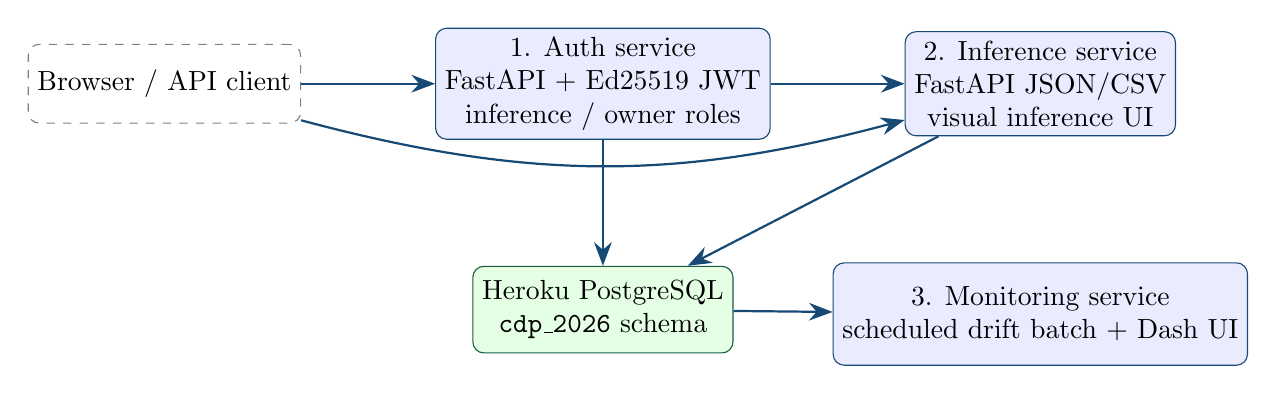
\begin{tikzpicture}[
  node distance=1.2cm and 1.7cm,
  service/.style={rectangle,rounded corners,draw=creditblue,fill=blue!8,minimum width=3.0cm,minimum height=1.3cm,align=center},
  db/.style={rectangle,rounded corners,draw=creditgreen!70!black,fill=green!10,minimum width=3.2cm,minimum height=1.1cm,align=center},
  ext/.style={rectangle,rounded corners,dashed,draw=gray,minimum width=2.0cm,minimum height=1.0cm,align=center},
  arrow/.style={-{Stealth[length=3mm]},thick,draw=creditblue}]
  \node[ext] (client) {Browser / API client};
  \node[service,right=of client] (auth) {1. Auth service\\FastAPI + Ed25519 JWT\\inference / owner roles};
  \node[service,right=of auth] (api) {2. Inference service\\FastAPI JSON/CSV\\visual inference UI};
  \node[service,below=1.6cm of api] (monitor) {3. Monitoring service\\scheduled drift batch + Dash UI};
  \node[db,below=1.6cm of auth] (postgres) {Heroku PostgreSQL\\\texttt{cdp\_2026} schema};
  \draw[arrow] (client)--(auth); \draw[arrow] (client) to[bend right=15] (api);
  \draw[arrow] (auth)--(api); \draw[arrow] (auth)--(postgres); \draw[arrow] (api)--(postgres); \draw[arrow] (postgres)--(monitor);
\end{tikzpicture}}
\end{center}
\vspace{0.15cm}
\small Stack: Python, FastAPI, Dash, SQLAlchemy, PostgreSQL 17, Docker, Heroku Container Registry, GitHub Actions and SonarCloud. Monitoring is one logical service deployed as separate batch and UI processes for operational isolation.
\end{frame}

\begin{frame}{Drift-monitoring showcase result}
\begin{columns}[T]
\column{0.52\textwidth}
\begin{block}{Forced seven-day window}
\begin{itemize}
  \item 120 deliberately shifted synthetic rows sent through normal inference validation, idempotency and PostgreSQL logging.
  \item 121 prediction rows analyzed after catch-up processing.
  \item 46 aggregate monitoring metrics: \textbf{22 ok}, \textbf{19 alert}, \textbf{4 warning}, \textbf{1 insufficient data}.
  \item Mean default probability: 0.075477; all 120 showcase decisions were on-time.
\end{itemize}
\end{block}
\column{0.43\textwidth}
\begin{block}{Correct interpretation}
The shifted batch demonstrates that feature/score drift and data-quality alerts work. It is \textbf{not} model-validation evidence. Performance/calibration stay ``insufficient data'' until mature outcomes arrive.
\end{block}
\end{columns}
\end{frame}

\begin{frame}{SAST findings: context and remediation}
\begin{columns}[T]
\column{0.49\textwidth}
\textbf{S8544 - dependency locking}\vspace{0.1cm}
\begin{itemize}
  \item Service requirement files use exact validated versions (for example FastAPI, SQLAlchemy, XGBoost CPU).
  \item The screenshot is historical; dependency versions are now pinned per service image.
  \item Remaining improvement: add hash-locked generated constraints when supply-chain policy requires artifact integrity verification.
\end{itemize}
\column{0.49\textwidth}
\textbf{S8707 - path traversal through CLI path}\vspace{0.1cm}
\begin{itemize}
  \item This was remediated, not dismissed as a false positive.
  \item The installer no longer accepts a file path from \texttt{sys.argv}; it reads only its co-located, repository-owned deployment contract.
  \item The trusted CI environment reduces exposure, but removing unnecessary input is the durable control.
\end{itemize}
\end{columns}
\vspace{0.25cm}
\begin{block}{Evidence to add before delivery}
Insert the SonarCloud screenshots: resolved S8544 and closed S8707 finding.
\end{block}
\end{frame}

\begin{frame}{Takeaways and next steps}
\begin{itemize}
  \item The pipeline is reproducible, CPU-deployable and separated from local CUDA experimentation.
  \item Production captures inference events safely and calculates aggregate drift/performance with explicit insufficient-data states.
  \item The branch and PR history makes engineering review auditable from EDA through production.
  \item Next: settle the explicit XGBoost-versus-LightGBM tie-break policy, collect matured outcomes, and replace deck placeholders with review/Sonar screenshots.
\end{itemize}
\vfill
\centering\Large Questions
\end{frame}

\end{document}
